% \def\bmode{1} % Mode 0 for presentation, mode 1 (or not 0) for a handout.
% \if 0\bmode
% 	\documentclass[smaller]{beamer}
% \else
% 	\documentclass[smaller,handout]{beamer}
% 	\usepackage{handoutWithNotes}
% 	\pgfpagesuselayout{2 on 1 with notes}[letterpaper, landscape, border shrink=4mm] 
% \fi

\documentclass[smaller,handout
]{beamer}
%\usepackage{handoutWithNotes}
%\pgfpagesuselayout{2 on 1 with notes}[letterpaper, landscape, border shrink=4mm]

% \documentclass[smaller,handout
% ]{beamer}
%\usepackage{etex}
%\newcommand{\num}{6{} }

% \usetheme[
%   outer/progressbar=foot,
%   outer/numbering=counter,
%  block=fill
% ]{metropolis}

%\useoutertheme{metropolis}

\usetheme{Madrid}
\useoutertheme[subsection=false]{miniframes} % Alternatively: miniframes, infolines, split
\useinnertheme{circles}
\usecolortheme{seahorse}

\usepackage[backend=biber,style=authoryear,maxcitenames=2,maxbibnames=99,safeinputenc,url=false,
eprint=false]{biblatex}
\addbibresource{bib/references.bib}
\AtEveryCitekey{\iffootnote{{\tiny}\tiny}{\tiny}}
\usepackage{svg}
%\usepackage{pgfpages}
%\setbeameroption{hide notes} % Only slides
%\setbeameroption{show only notes} % Only notes
%\setbeameroption{hide notes} % Only notes
%\setbeameroption{show notes on second screen=right} % Both

% \usepackage[sfdefault]{Fira Sans}

% \setsansfont[BoldFont={Fira Sans}]{Fira Sans Light}
% \setmonofont{Fira Mono}

%\usepackage{fira}
%\setsansfont{Fira}
%\setmonofont{Fira Mono}
% To give a presentation with the Skim reader (http://skim-app.sourceforge.net) on OSX so
% that you see the notes on your laptop and the slides on the projector, do the following:
% 
% 1. Generate just the presentation (hide notes) and save to slides.pdf
% 2. Generate onlt the notes (show only nodes) and save to notes.pdf
% 3. With Skim open both slides.pdf and notes.pdf
% 4. Click on slides.pdf to bring it to front.
% 5. In Skim, under "View -> Presentation Option -> Synhcronized Noted Document"
%    select notes.pdf.
% 6. Now as you move around in slides.pdf the notes.pdf file will follow you.
% 7. Arrange windows so that notes.pdf is in full screen mode on your laptop
%    and slides.pdf is in presentation mode on the projector.

% Give a slight yellow tint to the notes page
%\setbeamertemplate{note page}{\pagecolor{yellow!5}\insertnote}\usepackage{palatino}


%\usetheme{metropolis}
%\usecolortheme{beaver}
%\usepackage{xcolor}
\definecolor{darkcandyapplered}{HTML}{A40000}
\definecolor{lightcandyapplered}{HTML}{e74c3c}

%\setbeamercolor{title}{fg=darkcandyapplered}
%\setbeamercolor{frametitle}{bg=darkcandyapplered!80!black!90!white}
%\setbeamertemplate{frametitle}{\bf\insertframetitle}
%\setbeamercolor{footnote mark}{fg=darkcandyapplered}
%\setbeamercolor{footnote}{fg=darkcandyapplered!70}
%\Raggedbottom
%\setbeamerfont{page number in head/foot}{size=\tiny}
%\usepackage[tracking]{microtype}


\setbeamertemplate{frametitle}{%
    \nointerlineskip%
    \begin{beamercolorbox}[wd=\paperwidth,ht=2.0ex,dp=0.6ex]{frametitle}
        \hspace*{1ex}\insertframetitle%
    \end{beamercolorbox}%
}



\setbeamerfont{caption}{size=\footnotesize}
\setbeamercolor{caption name}{fg=darkcandyapplered}


%\usepackage[sc,osf]{mathpazo}   % With old-style figures and real smallcaps.
%\linespread{1.025}              % Palatino leads a little more leading

% Euler for math and numbers
%\usepackage[euler-digits,small]{eulervm}
%\AtBeginDocument{\renewcommand{\hbar}{\hslash}}
\usepackage{graphicx,multirow,paralist,booktabs}


%\mode<presentation> { \setbeamercovered{transparent} }

\setbeamertemplate{navigation symbols}{}
\makeatletter
\def\beamerorig@set@color{%
  \pdfliteral{\current@color}%
  \aftergroup\reset@color
}
\def\beamerorig@reset@color{\pdfliteral{\current@color}}
\makeatother

%=== GRAPHICS PATH ===========
\graphicspath{{./m1-images/}}
% Marginpar width
%Marginpar width
%\setlength{\marginparsep}{.02in}


%% Captions
% \usepackage{caption}
% \captionsetup{
%   labelsep=quad,
%   justification=raggedright,
%   labelfont=sc
% }

%AMS-TeX packages

\usepackage{amssymb,amsmath,amsthm} 
\usepackage{bm}
\usepackage{color}

\usepackage{hyperref,enumerate}
\usepackage{minitoc,array}


%https://tex.stackexchange.com/a/31370/2269
\usepackage{mathtools,cancel}

\renewcommand{\CancelColor}{\color{red}} %change cancel color to red

\makeatletter
\let\my@cancelto\cancelto %copy over the original cancelto command
\newcommand<>{\cancelto}[2]{\alt#3{\my@cancelto{#1}{#2}}{\mathrlap{#2}\phantom{\my@cancelto{#1}{#2}}}}
% redefine the cancelto command, using \phantom to assure that the
% result doesn't wiggle up and down with and without the arrow
\makeatother


\definecolor{slblue}{rgb}{0,.3,.62}
\hypersetup{
    colorlinks,%
    citecolor=blue,%
    filecolor=blue,%
    linkcolor=blue,
    urlcolor=slblue
}

%%%TIKZ
\usepackage{tikz}
\usepackage{pgfplots}
\usepackage{pgfplotstable}
\usepackage{pgfgantt}
\pgfplotsset{compat=newest}

\usetikzlibrary{arrows,shapes,positioning,shapes.geometric}
\usetikzlibrary{decorations.markings}
\usetikzlibrary{shadows,automata}
\usetikzlibrary{patterns}
\usetikzlibrary{trees,mindmap,backgrounds}
%\usetikzlibrary{circuits.ee.IEC}
\usetikzlibrary{decorations.text}
% For Sagnac Picture
\usetikzlibrary{%
    decorations.pathreplacing,%
    decorations.pathmorphing%
}
\tikzset{no shadows/.style={general shadow/.style=}}
%
%\usepackage{paralist}


%%% FORMAT PYTHON CODE
%\usepackage{listings}
% Default fixed font does not support bold face
\DeclareFixedFont{\ttb}{T1}{txtt}{bx}{n}{8} % for bold
\DeclareFixedFont{\ttm}{T1}{txtt}{m}{n}{8}  % for normal

% Custom colors
\definecolor{deepblue}{rgb}{0,0,0.5}
\definecolor{deepred}{rgb}{0.6,0,0}
\definecolor{deepgreen}{rgb}{0,0.5,0}

%\usepackage{listings}

% Python style for highlighting
% \newcommand\pythonstyle{\lstset{
% language=Python,
% basicstyle=\footnotesize\ttm,
% otherkeywords={self},             % Add keywords here
% keywordstyle=\footnotesize\ttb\color{deepblue},
% emph={MyClass,__init__},          % Custom highlighting
% emphstyle=\footnotesize\ttb\color{deepred},    % Custom highlighting style
% stringstyle=\color{deepgreen},
% frame=tb,                         % Any extra options here
    % showstringspaces=false            % 
% }}

% % Python environment
% \lstnewenvironment{python}[1][]
% {
% \pythonstyle
% \lstset{#1}
% }
% {}

% % Python for external files
% \newcommand\pythonexternal[2][]{{
% \pythonstyle
% \lstinputlisting[#1]{#2}}}

% Python for inline
% 
% \newcommand\pythoninline[1]{{\pythonstyle\lstinline!#1!}}


\newcommand{\osn}{\oldstylenums}
\newcommand{\dg}{^{\circ}}
\newcommand{\lt}{\left}
\newcommand{\rt}{\right}
\newcommand{\pt}{\phantom}
\newcommand{\tf}{\therefore}
\newcommand{\?}{\stackrel{?}{=}}
\newcommand{\fr}{\frac}
\newcommand{\dfr}{\dfrac}
\newcommand{\ul}{\underline}
\newcommand{\tn}{\tabularnewline}
\newcommand{\nl}{\newline}
\newcommand\relph[1]{\mathrel{\phantom{#1}}}
\newcommand{\cm}{\checkmark}
\newcommand{\ol}{\overline}
\newcommand{\rd}{\color{red}}
\newcommand{\bl}{\color{blue}}
\newcommand{\pl}{\color{purple}}
\newcommand{\og}{\color{orange!90!black}}
\newcommand{\gr}{\color{green!40!black}}
\newcommand{\nin}{\noindent}
\newcommand{\la}{\lambda}
\renewcommand{\th}{\theta}
\newcommand{\al}{\alpha}
\newcommand{\G}{\Gamma}
\newcommand*\circled[1]{\tikz[baseline=(char.base)]{
            \node[shape=circle,draw,thick,inner sep=1pt] (char) {\small #1};}}

\newcommand{\bc}{\begin{compactenum}[\quad--]}
\newcommand{\ec}{\end{compactenum}}

\newcommand{\p}{\partial}
\newcommand{\pd}[2]{\frac{\partial{#1}}{\partial{#2}}}
\newcommand{\dpd}[2]{\dfrac{\partial{#1}}{\partial{#2}}}
\newcommand{\pdd}[2]{\frac{\partial^2{#1}}{\partial{#2}^2}}



%%%%%%%%%%%%%%%%%%%%%%%%%%%%%%%%%%%%%%%%%%%%%%%%%%%
%%%%%%%%%%%%%%%%%%%%%%%%%%%%%%%%%%%%%%%%%%%%%%%%%%%

\title[CEE 260/MIE 273 M1c: Case Studies]{{\normalsize CEE 260/MIE 273: Probability and Statistics in Civil Engineering} \\
M1c: Case studies and experiments}\date[\today]{\footnotesize \today}
\author{{\bf Prof.\ Oke}}
\institute[UMass Amherst]{
  \begin{tikzpicture}[baseline=(current bounding box.center)]
    \node[anchor=base] at (-7,0) (its) {\includegraphics[scale=.3]{UMassEngineering_vert}} ;
  \end{tikzpicture}
}



%https://tex.stackexchange.com/questions/55806/mindmap-tikzpicture-in-beamer-reveal-step-by-step
  % \tikzset{
  %   invisible/.style={opacity=0},
  %   visible on/.style={alt={#1{}{invisible}}},
  %   alt/.code args={<#1>#2#3}{%
  %     \alt<#1>{\pgfkeysalso{#2}}{\pgfkeysalso{#3}} % \pgfkeysalso doesn't change the path
  %   },
  % }


% \usepackage{listings}

% \lstset{language=matlab,
%                 basicstyle=\scriptsize\ttfamily,
%                 keywordstyle=\color{blue}\ttfamily,
%                 stringstyle=\color{blue}\ttfamily,
%                 commentstyle=\color{gray}\ttfamily,
%                 morecomment=[l][\color{gray}]{\#}
%               }
         
\begin{document}

\maketitle




\begin{frame}
  \frametitle{Outline}
  \tableofcontents
\end{frame}


% \begin{frame}
%   \frametitle{Recap from Lecture 1a}
%   \begin{itemize}
%   \item Two categories of uncertainty: aleatory and epistemic
%   \item Visualize distributions via histograms and scattegrams
%   \item Measures of location: mean, median, mode
%   \item Measures of dispersion: range, variance, standard deviation, coefficient of variation
%   \end{itemize}
% \end{frame}

% \begin{frame}
%   \frametitle{Objectives of today's lecture}
%   \pause

%   \begin{itemize}[<+->]
%   \item Understand quantiles and boxplots

%   \item Learn how to use MATLAB to generate descriptive statistics and graphical summaries of datasets
%   \end{itemize}
% \end{frame}


% \section{Survey Results}
 

% \begin{frame}
%   \frametitle{Class expectations (Fall 2020)}
%   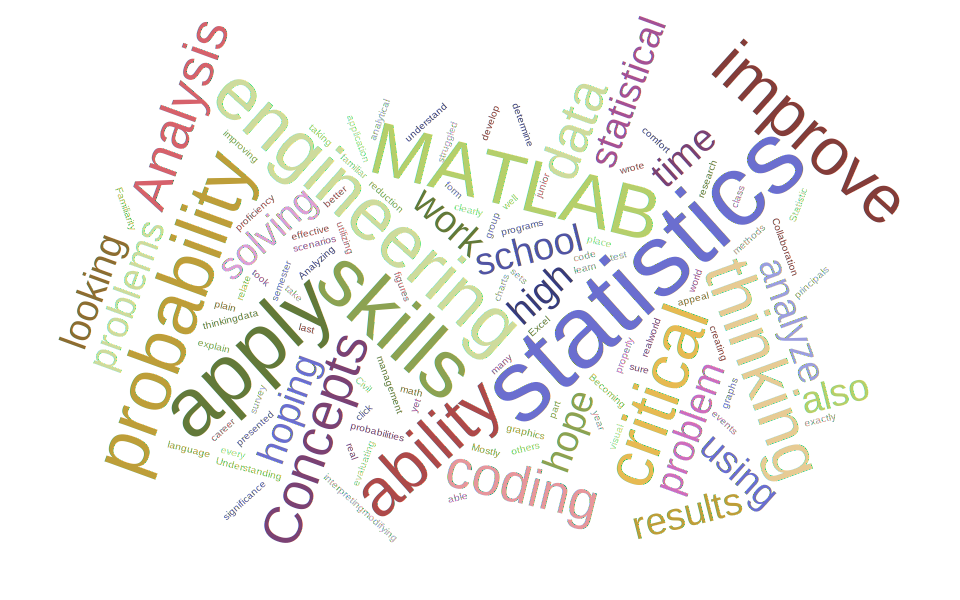
\includegraphics[width=\textwidth]{wordcloud2020}
% \end{frame}

% \begin{frame}
%   \frametitle{Your expectations (Fall 2021)}
%   \includegraphics[width=\textwidth,trim={2in 2in 2in 2in},clip]{wordcloud2021}
% \end{frame}

\begin{frame}
  \frametitle{Your expectations (Fall 2025)}
  \includegraphics[width=\textwidth]{wordcloud2025}
\end{frame}




\section{Recap: Quantiles and boxplots}
\begin{frame}
  \frametitle{Quantiles}
  \pause

  Quantiles are cutoff points that partition an ordered sample or dataset into equal-sized groups. \pause


  \begin{itemize}[<+->]
  \item A \textbf{median} splits a sample into two: $m$
  \item Two \textbf{terciles} split a sample into 3 groups: $T_{1}, T_{2}$
  \item Three \textbf{quartiles} split a sample into 4 groups: $Q_{1}, Q_{2}, Q_{3}$
  \item Four \textbf{quintiles} split a sample into 5 groups: $QU_{1}, QU_{2}, QU_{3}, QU_{4}$
  \item \dots
  \item Ninety-nine \textbf{[per]centiles} split a sample into 100 groups: $P_{1}, \ldots, P_{99}$
  \end{itemize}

\end{frame}


\begin{frame}
  \frametitle{Quantiles (cont.)} \pause
  Certain quantiles are equivalent to others: \pause

  \bigskip
  
  \begin{center}
  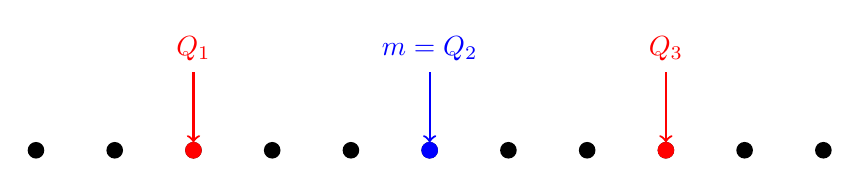
\begin{tikzpicture}
    \only<+->{\foreach \point in {(0,0),(1,0),(2,0),(3,0), (4,0), (5,0), (6,0), (7,0), (8,0), (9,0), (10,0)}{% points
      \fill \point circle (3pt);
    }}

    \only<+->{\draw[<-, thick, blue] (5,0.1) -- (5,1) node[above] {$m = Q_{2}$};
    \fill[blue] (5,0) circle (3pt);}
    \only<+->{\draw[<-,red, thick] (2,0.1) -- (2,1) node[above] {$ Q_{1}$};
      \draw[<-, red, thick] (8,0.1) -- (8,1) node[above] {$ Q_{3}$};
        \fill[red] (2,0) circle (3pt);
    \fill[red] (8,0) circle (3pt);}
  \end{tikzpicture}

  \pause
    
\end{center}
\pause

\bigskip

  \begin{itemize}[<+->]
  \item The median is the second quartile $Q_{2}$
  \item The 25th percentile is equivalent to the first quartile $Q_{1}$
  \end{itemize}

  \begin{exampleblock}{}
    Sextiles ($S_{1}, S_{2}, \ldots)$ partition a distribution into 6 equal groups.
    \begin{enumerate}[<+->]
    \item How many sextiles are there? %% 
    \item The second sextile $S_{2}$ can be expressed as which tercile?\footnote{Recall that a tercile splits a sample into 3 equal groups.}
    \end{enumerate}
    \pause
    {\gr Answers: Q1: There are 5 sextiles; Q2: $S_{2} = T_{1}$ (first tercile)}
  \end{exampleblock}
%\begin{quote}
  %   When presenting or analysing measurements of a continuous variable it is
  %   sometimes helpful to group subjects into several equal groups. For example,
  %   to create four equal groups we need the values that split the data such that
  %   25\% of the observations are in each group.\pause The cut off points are called
  %   \textbf{quartiles}, and there are three of them (the middle one also being called the
  %   \textbf{median}).\pause Likewise, we use two \textbf{tertiles} to split data into three groups, four
  %   \textbf{quintiles} to split them into five groups, and so on.\pause The general term for
  %   such cut off points is \textbf{quantiles}; other values likely to be encountered are
  %   \textbf{deciles}, which split data into 10 parts, and \textbf{[per]centiles}, which split the data
  %   into 100 parts. Values such as quartiles can also
  %   be expressed as centiles; for example, the lowest quartile is also the 25th
  %   centile and the median is the 50th centile.\footnote{ BMJ 1994;309:996 \url{https://www.bmj.com/content/309/6960/996}}
  % \end{quote}
\end{frame}



\begin{frame}
  \frametitle{Using boxplots}\pause

 % \begin{minipage}[t]{.45\linewidth}
  A boxplot\footnote{\tiny Figure source:
    \url{https://towardsdatascience.com/understanding-boxplots-5e2df7bcbd51}}
  displays the distribution of data\pause
    \begin{itemize}[<+->]
    \item Useful for identifying outliers
    \item Efficient for comparing multiple datasets
    \item The lines indicating the ``maximum/minimum'' points (excluding outliers) are called \textit{\rd whiskers}
    \end{itemize}

    \begin{center}
    \includegraphics[width=.8\textwidth]{boxplot}
  \end{center}
%  \end{minipage}
\end{frame}




\section{Colab Examples}
\begin{frame}
  \frametitle{Google Colaboratory}

  \pause

  \bigskip
  
  We will begin our introduction to Python via basic statistical analyses using the Google Colab platform (\url{https://colab.google/}).
  \pause

  \bigskip

  
  For an introduction, visit: \url{https://www.mathworks.com/help/matlab/getting-started-with-matlab.html}.
\end{frame}

\begin{frame}
  \frametitle{Notebooks}
  \pause

  Today, we will use the following Notebooks:

  \pause

  \begin{itemize}
  \item \texttt{m1-blind-stork.ipynb} \url{https://colab.research.google.com/drive/1G2_UPPli1rdfWv_9wRJvT-m2kLwg3GFu?usp=sharing}
    
  \item \texttt{m1-usa-housing.ipynb} \url{https://colab.research.google.com/drive/1onpllyTzNuoO9op89WDR4ft7o_U-eJVL?usp=sharing}
  \end{itemize}
\end{frame}

\begin{frame}
  \frametitle{Bonus Example}\pause
  \begin{exampleblock}{Example 1: Walking cadence}\pause
    In the article ``Can We Really Walk Straight?'' ({\it Amer. J. of Physical
      Anthropology}, 1992: 19--27) reported on an experiment in which each of 20
    healthy men was asked to walk as straight as possible to a target 60m away
    at normal speed.\\

    \bigskip
    \pause
    
    Consider the following observations on cadence (number of
    strides per second):

    \pause
    
    \begin{quote}\small
      .95 .85 .92 .95 .93 .86 1.00 .92 .85 .81 .78 .93 .93 1.05 .93 1.06 .96 .81 .96
    \end{quote}
    \pause
    \bigskip
    
    {\it Summarize the data; interpret and discuss.}
  \end{exampleblock}
\end{frame}


% \begin{frame}
%   \frametitle{Summarizing data: stem-and-leaf plots}\pause A stem-and-leaf plot shows
%   the frequency of defined interval using the actual values.
  
%   \begin{exampleblock}{Example 2: Active repair time}\pause
%     Consider the following data on active repair time (hours) for a sample of
%     $n=46$ airborne communications receivers: \pause
%     \begin{quote}
%       .2 .3 .5 .5 .6 .6 .7 .7 .7 .8 .8 .8 1.0 1.0 1.0 1.0 1.1 1.3 1.5 1.5 1.5
%       1.5 2.0 2.0 2.2 2.5 2.7 3.0 3.0 3.3 3.3 4.0 4.0 4.5 4.7 5.0 5.4 5.4 7.0
%       7.5 8.8 9.0 10.3 22.0 24.5
%     \end{quote}
%     \pause
%     {\it Construct (a) A stem-and-leaf display, and (b) A histogram based on
%       six class intervals with 0 as the lower limit of the first interval and
%       interval widths of 2, 2, 2, 4, 10, and 10 respectively.}
%   \end{exampleblock}
% \end{frame}

\begin{frame}
  \frametitle{To be assigned: Iris dataset}
  We will explore the properties and applications of boxplots using the following datasets:\pause
  \bigskip
  
  \begin{itemize}[<+->]
  \item  Popularized in Ronald A. Fisher's classic 1936 paper, ``The Use of Multiple Measurements in Taxonomic Problems'' \url{https://onlinelibrary.wiley.com/doi/10.1111/j.1469-1809.1936.tb02137.x}

  \item Data collected by Edgar Anderson on various measurements of 3 species of Iris flowers

  \item Also found on the UCI Machine Learning Repository. Data available by default on MATLAB
  \end{itemize}
  
\end{frame}


\begin{frame}
  \frametitle{Example 2: Iris species}
  \pause
  
  Three species of the \textit{Iris} flower:
  \pause
  
  \begin{figure}[h!]
    \centering
    \includegraphics[width=\textwidth]{iris-species}
    \caption{Iris species {\tiny (Source:
        \url{https://s3.amazonaws.com/assets.datacamp.com/blog_assets/Machine+Learning+R/iris-machinelearning.png)}}}
  \end{figure}
\end{frame}

% \begin{frame}
%   \frametitle{Example 2: Iris flower measurements}
%   \pause

%   \begin{figure}[h!]
%     \centering
%     \includegraphics[width=.3\textwidth]{iris-measurements}
%     \caption{\textit{Iris versicolor} sepal and petal measurements {\tiny (Source: \url{https://yculz33w9skgdkhey8rajqm6-wpengine.netdna-ssl.com/wp-content/uploads/2018/11/versicolor.jpg) }}}
%   \end{figure}

%   \pause
  
%   Are there significant differences in the petal/sepal width/length in each species?
% \end{frame}


% \begin{frame}
%   \frametitle{Example 3: ``Daphne and Santa Cruz.''}
  
%   \begin{itemize}[<+->]
%   \item The data set consists of measurements of beak sizes in mm of one species
%     of Darwin's ground finch (Geospiza fortis) taken at Daphne Island and at
%     Santa Cruz Island in the Galapagos by Peter and Rosemary Grant.

%     \item Data was extracted from 
%       \url{http://wps.prenhall.com/esm_freeman_evol_3/0,8018,8412374-,00.html}.

%       \item The
%       original data is summarized in the article: ``The classical case of
%       character release: Darwin's finches (Geospiza) on Isla Daphne Major,
%       Galapagos'' by P. T. Boag and P. R. Grant that appeared in Biological
%       Journal of the Linnean Society 22:243-287 (1984).
%   \end{itemize}
% \end{frame}


\section{Outlook}
\begin{frame}
  \frametitle{Recap}
  \begin{itemize}[<+->]
  \item Pre-survey review
  \item Python/Colab Introduction:
    \begin{itemize}
    \item Summarizing data
    \item Visualizing data: histograms, boxplots
    \end{itemize}
  \end{itemize}
\end{frame}

\begin{frame}
  \frametitle{Problem Sets}
  \pause

  \begin{itemize}[<+->]
  \item PS1 due at 1pm today
  \item PS2 will be assigned this afternoon
  \end{itemize}
\end{frame}



%\begin{frame}[allowframebreaks]
%   \frametitle{References}
%   \AtNextBibliography{\scriptsize}
%   \setbeamertemplate{bibliography item}[text]
%   \printbibliography[heading=none]
  
% \end{frame}

%\printbibliography
\end{document}
%%% Local Variables:
%%% mode: latex
%%% TeX-master: t
%%% End:
